\documentclass[11pt]{report}
\usepackage{baththesis}
\usepackage{graphicx}
\usepackage{caption}
\usepackage{amsmath}
\usepackage{latexsym}
\usepackage{multirow}
\usepackage{subcaption}
\usepackage{verbatim}
\usepackage[inline]{enumitem}
%\usepackage{amsfonts}
\usepackage{url}
\usepackage{natbib}
\usepackage[hmargin=3cm,vmargin=2cm]{geometry}
%\usepackage{mathpazo}
%\usepackage{eulervm}
\usepackage[usenames,dvipsnames,svgnames,table]{xcolor}
\usepackage[]{todonotes}
\usepackage{tikz}
\usetikzlibrary{arrows}
\usepackage[]{todonotes}

\def\mnote#1{\todo[color=Goldenrod,size=\scriptsize]{Matt: #1}}
\def\jnote#1{\todo[color=CornflowerBlue,size=\scriptsize]{Julian: #1}}
\def\snote#1{\todo[color=WildStrawberry,size=\scriptsize]{Steve: #1}}
\definecolor{light-gray}{gray}{0.95}

\usepackage{listings}
\lstset{ %
   language=prolog,
%  frame=l,                     % adds a frame around the code
   basicstyle=\footnotesize\ttfamily,  % use courier
   breaklines=true,
   xleftmargin=0.5em,
   aboveskip=0.5em,
   belowskip=0.5em,
%  belowcaptionskip=5em,
   numbers=left,
   backgroundcolor=\color{light-gray},
   frame=single,
   framerule=0pt
}

\setlength{\jot}{0pt}
\def\mylabel#1{\tikz[remember picture]\node(#1){};}
\def\myref#1#2#3{\begin{tikzpicture}[remember picture]
\node[draw,rounded corners] (#2){\begin{minipage}{\textwidth}\raggedright#3\end{minipage}};
\draw[overlay,-triangle 45,thick,gray](#2.west)--(#1.west);
\end{tikzpicture}}

\title{Building Abstractable Story Components with Institutions and Tropes}
\author{Matt Thompson}
\degree{EngD Digital Media}
\department{Department of Computer Science}
\degreemonthyear{October 2016}
\norestrictions


\begin{document}
\maketitle
\clearpage
\tableofcontents
\clearpage

\chapter{Introduction}
\label{cha:introduction}
This report summarises the research carried out as part of the EngD Digital Media programme with the University of Bath and Sysemia Ltd.

The purpose of this report is to explain the academic research conducted during the course and its applicability to the needs of Sysemia Ltd. The main focus is to explore the state of the art in interactive and generative narrative and also to apply it in a real-world exhibition context.

Interactive narratives have the potential to transform two major fields: games
and training simulations. These are the applications for which the use of
interactive narrative can benefit Sysemia. The main part of the research examines the state of the art in interactive narrative primarily in computer games research, but then adapts techniques from that field for the purpose of interactive exhibitions for education. By implementing research ideas into `toy' game projects (such as an interactive Punch and Judy show in section \ref{}), I then take components from these projects and implement them into practical exhibition-based projects for Sysemia (such as the Every Object Tells a Story project described in section \ref{}).

\section{Interactive narrative for games}
Computer games are a new medium for artistic expression. The element of interactivity, combined with visual art, music and storytelling, allows the creation of ever more fantastic worlds. This combination of previous art forms isn't enough, though. Game creators are now experimenting with ways to make a narrative itself interactive. Imagine playing through a version of Romeo and Juliet where there is a possibility that the characters could escape their fates. Or playing a detective in a game where the story changes depending on how quickly you can piece together clues.

This is the new frontier that we are exploring with this research: the as-yet unconquered domain of \emph{interactive} storytelling.

We are defined by the choices we make throughout our lives. These choices form a story that describes our own personal history. If a player can watch somebody's life unfold and witness the choices that they made, and those that were forced upon them, they would have a deep understanding of how they came to be who they are.

This kind of deep understanding is only possible through experiencing a story where the decisions made have real consequences. Traditional fiction, and perhaps computer games, enable this to some extent. But the story is still experienced passively by the consumer in these media. A truly interactive narrative would go deeper, as though you had truly lived as another person.

For this reason, interactive narrative for games is worth exploring: it would
enable a player to truly understand other people's lives and situations, and why they became the people they are.

% Put a bit about what you did to explore the potential of interactive narrative
% for games

\section{Interactive narrative for education}
Stories are a powerful way for humans to understand and remember facts and events. Making these stories interactive could lead the way to even more effective learning methods.

\citet{schank1990tell} argues that stories may be a useful way for humans to better remember a series of events, when compared to simply reciting them as a list of facts. Mentalists and creative students use storytelling mnemonic techniques to help them memorise large lists of difficult-to-remember facts with perfect recall.

Training simulations make the use of stories taking place in immersive environments to help trainees to master new routines and techniques. These stories always follow a fixed pattern, however, unlike the mnemonic stories that people create to memorise information, which are highly personalised to the practitioner.

A narrative that dynamically reacts to the decisions of the audience could better enable them to remember information when compared with a static, unpersonalised narrative.

With this in mind, it is worth constructing an interactive narrative system and applying it to both entertainment and learning contexts. Some evaluation still needs to be carried out in order to determine how much more effective (if at all) interactive narrative could be for education, so this is proposed as part of this report.

Preliminary work has been done in collaboration with the Bishop's Palace in Wells to create an exhibition incorporating interactive narrative. Using a combination of Semantic Web data formats and an event calculus-based reasoner, the system will be able to infer future actions for recommendation to visitors. Description of the work done so far is in section \ref{}.

Both the game-based and education-based projects have a common thread: reasoning
over temporal data in order to predict future events, or constrain possible
future actions to conform to a narrative domain. Section \ref{}
describes the direction the research has taken, and how the use of techniques such as hierarchical institutions and the creation of an ontology for narrative might develop these ideas further.

\section{Outline}
% Outline of sections goes here
This thesis begins with a review of the literature in Section~\ref{cha:literature-review}. This review covers two main fields of research: narrative research from social science (Section~\ref{sec:narratology}), and interactive narrative research from computer science (Section~\ref{sec:implementations}).
The ``Institutions as Story Worlds'' chapter (\ref{cha:institutions}) describes the theory and research behind instituitions, and discusses the merit of their use for describing story, comparing their use against other logics and planner-based systems.
The ``Tropes as Story Components'' chapter (\ref{cha:tropes}), discusses the use
of \emph{tropes} as story components, and why they improve upon existing narrative formalisms.
Chapter~\ref{cha:tropes-and-institutions} describes how to use institutions to define tropes, and how to combine them to describe the story world for an interactive narrative. The section also describes the use of this technique to build a number of different narratives, contrasting the approach with using other techniques such as planners to build interactive narratives.
The final chapter looks back at the research done, evaluating its potential impact and discussing possible future work. 

\chapter{Literature Review}
\label{cha:literature-review}
This research covers a large number of fields of study, therefore an extensive
literature review covering these fields is needed. This section starts with a
look at the field of \emph{narratology}, or narrative theory, to gain some
insights into the themes and components that make up stories. Looking at
different formalisms that have been created for narrative and which themes and
motifs recur in stories should better inform the creation of techniques with
which to generate stories.

Additionally, computers have the potential to introduce a new type of storytelling. Though computer games offer increasingly immersive interactive worlds, the form of narrative they use remains much the same: linear. A player may be able to interact with elements of a game, but the story itself remains unchanged.
Chris Crawford refers to a new possible form of narrative as ``Interactive Storytelling'' \citep{crawford2012chris}. Though researchers and game designers have made great strides towards realising this new artform, little has been produced to capture the public imagination.

% why are you looking at classic narratology?
In order to better inform any implementation of interactive narrative, this
review begins with an examination of the field of classic narrative theory. Following from this is a look at the emerging research in interactive and generative narrative and their implementations.
As part of the examination of implementations of interactive narrative, this review especially focuses on agent-based systems. The section concludes with an overview of emotional models that can be used to model distinct characters using agents.

\section{Narratology}
\label{sec:narratology}
Narratology is a deep field with many sub-fields. This review examines the parts of it that might best inform the modelling of narrative by computers, as well as the construction of interactive narrative.

The first part of the overview of narratology examines research into categorising different types of narrative, both traditional and experimental.
This draws from classic narratological texts, as well as work done on ``cybertext'' and experimental narrative in the interactive age. This examination of recent research into non-linear narratives better informs how to better construct interactive narratives for games or simulations.

Structuralist formalisms of narrative attempt to explain how stories work by dividing them into commonly occuring themes and motifs. This is a natural fit to the modelling of narratives by computer, especially if using an ontology. This overview of narratology starts with structuralism for this reason.

After the overview of the structuralists follows a section on the use of formal logic for narrative modelling. The section ends with descriptions of other types of story components, taxonomies and ontologies used in the literature.

\subsection{Types of Narrative}
% Look at Cybertext, etc, and try to explain how best to divide different types
% of story
The rise of the Web in the 1990s brought with it great interest in the future of narrative in cyberspace. Aarseth's work, \emph{Cybertext} \citep{aarseth1997cybertext} describes the creation of a new form of narrative, for which he coins the term \emph{ergodic literature} (from the Greek words \emph{ergon} and \emph{hodos}, meaning `work' and `path'). In this new form of narrative, some amount of work or effort is required by the reader in order to traverse the path that the story takes.

% scriptons/discourse textons/fabula (Bal 1997)
Aarseth makes a distinction between the narrative as written by the author, and the way in which it is traversed by the reader, calling the former \emph{textons} and the latter \emph{scriptons}. In ergodic literature, the \emph{scripton} is produced by the effort that the reader goes through in interpreting the \emph{texton}. In the context of a game, it is as though the game interface is a gateway that allows access to the narrative at different times. Using classical music as a metaphor, the texton can be thought of as the \emph{score}, and the scripton the \emph{performance}.

% Make sure you actually made this assertion
In section \ref{sec:generative-and-interactive-narrative}, we assert that how generative a narrative is and its level of interactivity are two different variables in an experimental narrative. However, Aarseth identifies seven different methods of story traversal: \emph{dynamics, determinability, transiency, perspective, access, linking and user function}.

\paragraph{Dynamics} describe whether or not the content and number of scriptons changes. In a simple, static story with branching choices (such as in a \emph{Choose your own adventure} story), both the number of textons and scriptons are fixed, since all paths have been written out beforehand. A dynamic story would still have a fixed number of textons, but the scriptons would be generated as the user traverses the path of the narrative.
\paragraph{Determinability} is how deterministic the narrative is, whether or not the same interactions will result in the same scripton being produced.
\paragraph{Transiency} means to what extent scriptons are produced as time flows, or whether user interactions are required to produce them.
\paragraph{Perspective} is whether or not the user/reader plays a role as a character in the narrative.
\paragraph{Access:} if a user has access to all scriptons at any point in traversing the narrative, or whether their access is restricted.
\paragraph{Linking} means whether or not parts of the scripton are linked to other parts, and whether these links are conditional (if they rely on a user having already traversed part of the scripton).
\paragraph{User functions:} the functions the user uses to traverse the text. This could be interpretive (which is implicit in any traversal of the text), explorative (traversing the scripton according to whim) or configurative (specifying parts of the scripton in advance), for example.

% Ugh, this is all so arbitrary. Go on to describe Aarseth's PCA of these variables and explain why you don't think it's a good fit.

By performing correspondence analysis (a process similar to principle component analysis) on a diverse corpus of 23 texts ``\emph{ranging from ancient China to the Internet}'', Aarseth filters these seven variables down into two numerical axes which account for 49 percent of the variation between stories. Using these axes, he groups classic tales such as \emph{Moby Dick} and more experimental narratives such as William Gibson's \emph{Agrippa} and Michael Joyce's \emph{Afternoon}. By grouping these stories into categories, he intends to show how emerging media are enabling new types of story.

Chris Crawford's \emph{Chris Crawford on Interactive Storytelling} \citep{crawford2012chris} provides a scathing assessment of the relationship between narrative theory and computer science. A veteran of the games industry, he argues that `soft' science theories such as those of Aarseth et al are entirely removed from `hard' science, and are therefore an example of bubble intellectualism and impossible to implement. 

Crawford himself provides a useful examination of experimental narrative in computer games, defining interactivity as:

\begin{quote}
A cyclic process between two or more active agents in which each agent alternately listens, thinks, and speaks.
\end{quote}

He argues that for game narratives to be truly interactive, they must be more social. Characters in a story must be able to react with the player as though they were people in real life. In turn, the player should have some degree of freedom in the way in which they interact. Rather than presenting branching story points as choices, a better way to interact would be socially, through talking to agents in the game. This is the approach that Fa\c{c}ade takes \citep{mateas2003faccade}, which Crawford acknowledges as the most successful attempt at interactive storytelling to date. A detailed description of Fa\c{c}ade's implementation appears in section \ref{sec:modelling-agents}.

In order to determine whether Crawford's assertion that narratology research is too far removed from its practical implementations to be of use, we next provide an overview of these implementations and their underlying research. Has narrative theory research informed the creation of computer-generated or interactive narrative at all, or do they all take approaches grounded in computer science and artificial intelligence? If narrative theory has not been used, then we must ask another question: why not?


\subsection{Structuralist Formalisms of Narrative}
% Propp, etc
Attempts to organise recurring themes, roles and motifs of narrative go back at least a century. The Aarne-Thompson tale-type index \citep{aarne1987types}, first published in 1910 and later refined by Stith Thompson in 1928 and 1961, is well known amongst folklorists as a classification and analysis method for traditional folktales and myths. Aarne-Thompson's index is a taxonomy of tale themes, arranging tales into categories such as \emph{animal tales} and \emph{jokes and anecdotes}, and then sub-categories (\emph{tales of magic} and \emph{numskull [sic] stories} being two examples). This taxonomy is only two levels deep however, and only serves as a useful way to categorise individual stories or tales. In order to break down and analyse components of tales, we must dig deeper.

In \emph{Structural Anthropology}, Claude L\'{e}vi-Strauss seeks to discover why myths and legends are so similar across cultures and history \citep{levi2008structural}. He concludes that there are global laws that govern the way in which people create stories, therefore these laws can be modelled as a set of rules for describing myths.

His theory is that myths describe opposing forces which are resolved through mediation. The example he gives in \emph{Structural Anthropology} describes how Native American legends often contain `trickster' characters in the form of ravens or coyotes. As scavenging animals, these tricksters symbolically act as mediators between life and death.

Like much of early narrative theory, there is no rigorous evaluation of L\'{e}vi-Strauss' ideas, leaving them feeling a little too opinionated and arbitrary. While interesting, L\'{e}vi-Strauss' ideas bring us no closer to developing a formal model of narrative structure. For that, we must go even further back in time, and turn to Vladimir Propp.

\subsubsection{Propp's Morphology of the Folktale}
Propp's seminal work ``The Morphology of the Folktale'' \citep{propp1968morphology}, though first published in 1928, is still a widely-used formalism for researchers and game designers looking to generate narratives procedurally. Propp identifies recurring characters and motifs in Russian folklore, distilling them down to a concise set of rules with which to describe stories.

In this formalism, characters have \emph{roles}, such as \emph{hero}, \emph{villain}, \emph{dispatcher}, \emph{false hero}, and more. Characters performing a certain role are able to perform a subset of \emph{story functions}, which are actions that make the narrative progress. For example, the \emph{dispatcher} might send the \emph{hero} on a quest, or the \emph{victim} may issue an \emph{interdiction} to the \emph{villain}, which is then \emph{violated}.

Propp defines a total of 31 distinct story functions, each of which is given a number and symbol in order to create a succinct way of describing entire stories. Examples of such functions are:

\begin{itemize}
  \item One of the members of a family absents himself from home: \emph{absentation}.
  \item An interdiction is addressed to the hero: \emph{interdiction}.
  \item The victim submits to deception and thereby unwittingly helps his enemy: \emph{complicity}.
  \item The villain causes harm or injury to a member of the family: \emph{villainy}.
\end{itemize}

Each of these functions can vary to some degree. For example, the \emph{villainy} function can be realised as one of 19 distinct forms of villainous deed, including \emph{the villain abducts a person}, \emph{the villain seizes the daylight}, and \emph{the villain makes a threat of cannibalism}.

These functions are enacted by characters following certain roles. Each role (or \emph{dramatis personae} in Propp's definition) has a \emph{sphere of action} consisting of the functions that they are able to perform at any point in the story. Propp defines seven roles that have distict spheres of action: \emph{villain}, \emph{donor}, \emph{helper}, \emph{princess}, \emph{dispatcher}, \emph{hero}, and \emph{false hero}.

Though Propp defines each \emph{dramatis personae} as being distinct (characters can only play one role at a time), it is simple to extend the idea to allow for overlapping roles. For example, a victim could also be a donor, so the set of functions they can perform would be the union of both the victim and donors' permitted function sets. Propp does not explore this possibility in \emph{The Morphology of the Folktale}, however.

\begin{figure}[!t]
\centerline{
\includegraphics[height=0.4in]{propp1.png}}
\caption{One Propp function following another}\label{fig:propp1}
\end{figure}

\begin{figure}[!t]
\centerline{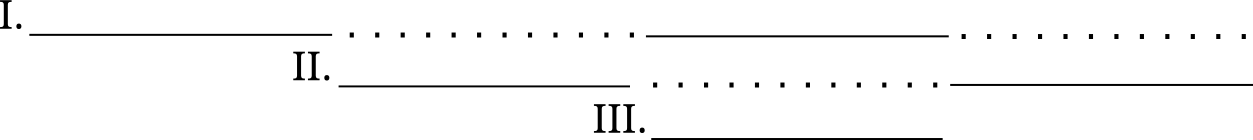
\includegraphics[height=0.6in]{propp2.png}}
\caption{Multiple simultaneous functions}\label{fig:propp2}
\end{figure}

In a typical story, one story function will follow another as the tale progresses in a sequential series of cause and effect (figure~\ref{fig:propp1}). However, Propp's formalism also allows for simultaneous story functions to be occuring at once (figure~\ref{fig:propp2}).

% What are the shortcomings of Propp? (i.e. lack of abstractability, etc)

\subsection{Describing Stories with Logic}
% Laure-Ryan did a bit of this

\subsection{Other Types of ``Story Component''}

\section{Implementations of Experimental Narrative}
\label{sec:implementations}
% I've plenty of material, but it really needs reworking and extending

\subsection{Story Generation}
% TaleSpin, etc

\subsubsection{Generative Grammar}

\subsubsection{Author Modelling}
% This would also use planners

% But this is limited in interactivity, so in order to have characters we can
% interact with, we must use...

\subsection{Intelligent Agents as Characters}
% Write an introduction


\paragraph{The OZ project}
Carnegie Mellon University's OZ project \citep{mateas1999oz} is one of the first major research efforts towards creating interactive drama using agents as characters. A dramatic structure is given to the narrative by means of a \emph{drama manager}, which is able to see all of the actions occurring in the storyworld and can change anything in order to create a better experience for the user.

Ideas from the OZ project were later developed into what would become Fa\c{c}ade.
% Facade, etc
\paragraph{Fa\c{c}ade}
Mateas and Stern's \emph{Fa\c{c}ade} has players interact with the characters of the story through natural language. In this game, the player attends the party of a young couple (Grace and Trip) celebrating their wedding anniversary. As the course of events unfold however, the player learns that all is not as happy as it seems.

The player interacts with the characters by typing in natural language sentences, to which Grace and Trip respond. Though the characters are implemented through agents, the story is controlled using a drama manager. In all, their system consists of using NLP, a novel character authoring language and a novel drama manager to create an interactive narrative.

Several custom-designed languages were used to create the game, including a language called `A Behaviour Language' (ABL) for the agents and a special language for the sequencing of the beats. ABL represents situations as character goals, maintaining a tree of all the active goals and behaviours that are happening at any time.

In Fa\c{c}ade, the smallest unit of narrative action is called a \emph{story beat}, taken from McKee's book on authorial style for screenwriters \citep{mckee1997substance}. The simulation constantly monitors what the user is doing and how it may lead from the current story beat to another. Story beats have preconditions and effects on the state of the narrative, so it is the drama manager's job to work out when it makes sense to initiate a certain beat.

`Beats' have a very fine granularity, with 200 or so updating every minute of the simulation. They consist of a set of ABL behaviours, which advance the narrative yet still allow interaction to change to other beats. Only one beat can be active at a time.

A beat can have 5 types of goal:

\begin{enumerate}
  \item transition-in: characters express their intentions
  \item body: a dramatic question/situation is posed to the player
  \item local/global mix-in: react to the player before end of the beat
  \item wait-with-timeout: wait for the player's reaction
  \item transition-out: final reaction to the player's action in the beat
\end{enumerate}

A beat goal is a series of steps for an agent to perform, which can be:

\begin{itemize}
  \item staging (where to walk to, face)
  \item dialogue to speak
  \item where and how to gaze
  \item arm gestures to perform
  \item facial expression to perform
  \item head and face gestures to perform
  \item small arm and head emphasis motions triggered by dialogue (head nods, hand flourishes)
\end{itemize}

As an example, there is a behaviour called ``Fix\_Drinks'', which specifies a sequence of agent behaviours where the characters Grace and Trip have an argument while Trip asks the player what they would like to drink. If the player decides not to go along with the beat (in this case, by not choosing a drink), then the beat will be aborted and replaced with another.

Fa\c{c}ade has become popular as a game outside of academia, with playthroughs of the game reaching millions of views on Youtube. This shows the promise of interactive narrative as being a unique and engaging new form of entertainment. Unfortunately, no other implementation of interactive narrative seems to have captured the public imagination since the release of Fa\c{c}ade.

Fa\c{c}ade's popularity seems to reinforce Crawford's assertion (section \ref{sec:media}) that interactive narratives must be social in nature. The gameplay comes entirely from the conversations and interactions between Grace, Trip and the player. Much of the excitement comes from the social consequences of certain conversation paths or actions. By modelling characters as agents, Mateas et al have created a truly interactive experience. However, by also using a drama manager to manage the agents, they have used these agents to tell a story.

How might these agents be made more convincing? Outside of writing rules for their behaviour consisting of character goals and beliefs, how might an author create truly unique and idiosyncratic characters? To address the question, I next examine different types of emotional models in psychology, and how each might be used to model characters as agents.

\subsubsection{Character Modelling}

\subsubsection{Characters with Emotional Models}
% Intro: not done very much?

\subsubsection{Emotional models}\label{sec:emotional-models}
% How is this useful for narrative?
Usually it would seem odd to want to model emotion as part of a computational process. Emotion is such a seemingly irrational set of behaviours that they are easy to dismiss as `human imperfections'. However, as \citet{marsella2014} observe, emotions may have a useful role to play in communication, so long as they are displayed at appropriate times.

For example, anger prepares the human body to fight by increasing the manufacture of adrenaline. Fear similarly triggers the `fight or flight' response, alerting the senses for danger and preparing the body to react.

In order to model human emotions using agents, we must first find a suitable psychological model to use. Marsella et al describe three main types of emotional model:

\begin{enumerate}
 \item \textbf{Discrete} emotional models, which claim that humans have a set of innate, pre-defined emotional states which people may enter and leave.
 \item \textbf{Dimensional} models of emotion, describing the spectrum of emotions as being points somewhere in continuous space. Implementations typically use two or three dimensions for simplicity.
 \item \textbf{Appraisal} theories of emotion take an agent's mental processes into account. Their emotional state is derived from whether or not their goals have been achieved, and what effects current events are having on their circumstances, for example.
\end{enumerate}

% Give examples of concrete models for each type.
\subsubsection{`Basic' emotions}
Ekman first made a case for discrete, biologically-determined emotions, based on evidence from research into facial expressions \citep{ekman1992argument}. He describes emotions as being \emph{basic}, in two senses of the word: \emph{i.} that there are a number of distinct emotions, each with its own different characteristics, and \emph{ii.} that these emotions were developed through evolution for specific functions.

Ekman argues that these evolved emotions share nine characteristics:

\begin{enumerate}
  \item Distinctive universal signals
  \item Presence in other primates
  \item Distinctive physiology
  \item Distinctive universals in antecedent events
  \item Coherence among emotional response
  \item Quick onset
  \item Brief duration
  \item Automatic appraisal
  \item Unbidden occurrence
\end{enumerate}

These characteristics are shared by all of the `basic' emotions as observed in humans and primates.

Discrete models of emotion suggest that there is a neural basis for emotion. For example, Armony et al describe how the amygdala in the brain is responsible for conditioned fear responses  and create a neural network to model it \citep{armony1997computational}.

Using a discrete model of emotion for agent-based characters would be relatively simple. Each basic emotion could have its own distinct set of behaviours as postconditions, and triggering circumstances as preconditions.

However, a more fluid approach could be useful when modelling emotions with agents. It would be impossible to say that an agent is \emph{angry and approaching furious} using a discrete theory of emotion. Nuanced levels of emotion and even combinations of several emotions add an extra level of texture to a character. Dimensional and appraisal theories of emotion address this challenge.

\subsubsection{Russell's circumplex model of emotion}\label{sec:circumplex}
\begin{figure}[!t]
\centerline{
\includegraphics[height=3in]{circumplex.png}}
\caption{Russell's circumplex model of emotion} \label{fig:circumplex}
\end{figure}

Russell's circumplex model of emotion is a well-known dimensional model \citep{russell1980circumplex}. In this case, the dimensional variables are \emph{valence} (how agreeable or otherwise a situation is to an agent) and \emph{arousal} (how excited an agent is).

Russell's original paper proposes a model similar to that shown in figure \ref{fig:circumplex}, where the $x$ axis is a person's valence level and the $y$ axis is their arousal level. He argues that the full range of human emotions lie as points along these axes. Eight such examples are shown in fig. \ref{fig:circumplex}.

This model is very easy to adapt to human-like agents. \citet{ahn2012nvc} adapt this model by adding a third dimension, dominance, to create conversational agents in a 3D environment. This `dominance' dimension was first proposed in Mehrabian and Russell's original work \citep{mehrabian1974approach}, but later removed due to being perceived as the consequences of the \emph{effects\/} of emotion \citep{russell1980circumplex}, rather than being a component of emotion itself. Like Ahn et al, I found it useful to add the dominance-submission dimension, and so left it in my emotional model. This is the approach I take in creating my Punch and Judy simulation, and so it is described in more detail in section \ref{sec:emotion}.

\subsubsection{Appraisal theory}
Appraisal theories of emotion lend well to simulation with agents, due to their taking a person's beliefs, desires and intentions into account with respect to external events. Emotions arise when an event occurs and a person internally \emph{appraises} its consequences with respect to their beliefs, desires and intentions. This fits well with the popular BDI architecture for intelligent agents.

Different methods of appraisal may be used in order to produce emotions. Gratch and Marsella use decision theoretic plans \citep{gratch2004domain}, but other approaches could include reactive plans, Markov-decision processes, or detailed cognitive models.

Though the Punch and Judy simulation described in section \ref{sec:punchjudy} uses a dimensional model of emotion, an appraisal-based model would be worth investigating due to its tight coupling with belief desire intention psychological models used in agents. I describe my intention to explore this area further in section \ref{sec:fappraisal}.


% But characters in a story need to follow some kind of underlying plot
% mechanism, so...

\subsection{Governing Narrative in a Multi-Agent System}
\subsubsection{Planner-based Systems}
% Riedl, Young, etc
\subsubsection{Social Norms}
Versu~\cite{evans2014versu} is an interactive drama system that uses a multi agent system as characters. The characters' actions are coordinated with \emph{social practices}, which describe types of social situations and is described by the authors as a successor to the Schankian script. These social practices are implemented as reactive joint plans, which agents can choose whether to participate in or not. Rather than directly telling the agents what to do, these social practices merely \emph{suggest} courses of action, leaving each agent to decide for itself what to do based on its individual goals.

The authors decide against using a drama manager to control the agents' actions because they want to take the \emph{strong autonomy} approach to agent governance. This means that they prefer to give each agent some degree of autonomy by allowing it to make the final decision on which course of action to take, rather than blindly following a drama manager. Suggesting actions with social norms achieves this goal. Rather than describing typical story events in terms of social norms, however, in Versu the social norms \emph{are} the story. The gameplay revolves around the avoidance (or purposeful subvertion of) awkward social situations.

Each character has a role, which is governed by a social practice. For example, a \emph{greeting} practice involves characters with the \emph{greeter} and recipient roles. The greeting practice would tell the greeter in which manner they are to greet the recipient, and the recipient how to respond. It is noteworthy that these actions are merely suggested, and not enforced.

\emph{Exclusion logic}~\cite{evans2010introducing}, a form of deontic logic, is used to describe the social practices of the system. Exclusion logic allows the description of tree structures and includes an exclusion operator.

For example, a description of a character called ``Brown'' is shown in listing \ref{lst:exclusive}. It describes the building up of character attributes as a tree structure.

\begin{lstlisting}[label=lst:exclusion,caption=Description of ``Brown'' character.]
brown.sex!male;
brown.class!upper;
brown.in!dining_room;
brown.relationship.lucy.evaluation.attractive!40;
brown.relationship.lucy.evaluation.humour!20.
\end{lstlisting}

Exclusion logic is designed to express the fact that a variable can only have one value. This saves the author from having to remember to change extra facts. For example, if the ``Brown'' character changes location from the dining room to the kitchen, \emph{brown.in!dining_room} is terminated when \emph{brown.in!kitchen} holds.

Versu takes the \emph{constitutive} view of social practice, as opposed to the \emph{regulative} view. This means that rather than restricting an agent's possible actions based on its permissions and obligations, they participate in a certain social practice by taking an action. Their actions are only restricted by what is possible in the story world, and what the agent desires to do. This way, agents can choose whether or not to take part in certain social interactions.

Many of the components we aim to have in our story telling system appear in Versu: the use of social norms to gently encourage story-conforming behaviour rather than demanding it, and the use of formal logic to determine which behaviours are possible. However in Versu the social norms \emph{are} the story, rather than describing the story components that invisibly govern the behaviour of characters. In order for this kind of governance to occur, an institution-based solution is preferable, based on events, agent actions and standard deontic logic. Because character actions are constrained by the structure of a story, a \emph{regulative}  view of social practice is more suited to the expression of story components as social norms.

Much of the advantages of using exclusion logic can be gained by using an institution-based approach. Non-inertial fluents can be used to ensure that variables can only ever have one value. Standard deontic logic is enough to provide the rest of what is needed.

\chapter{Institutions as Story Worlds}
\label{cha:institutions}

% Intro about justification/inspiration for using institutions for stories

\section{Describing Stories With Logic}
\subsection{Modal Logic and Kripke Structures}

\subsubsection{Propp Example: Sausages and Crocodile Scene}\label{sec:pjexample}
The common elements of Punch and Judy are easily described in terms of Propp's story functions. Here we pick one scene to use as an example: the scene where Punch battles a Crocodile in order to safeguard some sausages.  In this scene, Joey the clown (our narrator) asks Punch to guard the sausages. Once Joey has left the stage, a Crocodile appears and eats the sausages. Punch fights with the Crocodile, but it escapes. Joey then returns to find that his sausages are gone.
The corresponding story functions are:
\begin{enumerate}
  \item Joey tells Punch to look after the sausages (\emph{interdiction}).
  \item Joey has some reservations, but decides to trust Punch (\emph{complicity}).
  \item Joey gives the sausages to Punch (\emph{provision or receipt of a magical agent}).
  \item Joey leaves the stage (\emph{absentation}).
  \item A Crocodile enters the stage and eats the sausages (\emph{violation}).
  \item Punch fights with the Crocodile (\emph{struggle}).
  \item Joey returns to find that the sausages are gone (\emph{return}).
\end{enumerate}

Some story functions map to Punch and Judy better than others (for example, it is debatable as to whether or not the sausages can be considered a ``magical agent''), but Propp's formalism seems well suited to Punch and Judy for the most part. The advantage of using Propp for the Punch and Judy story domain is that the story function concept maps well to the idea of internal events in institutional models.

\subsubsection{Combining Interval Temporal Logic and Modal Logic for Propp}\label{sec:propplogic}
\mnote{Put in definitions as a footnote, Cyrillic if you want}
Narrative construction can be described using two terms: \emph{fabula} and \emph{syuzhet}. Fabula is the events of the story as they occur in chronological order, but syuzhet refers to those events as they are ordered in the story's telling. Fabula describes one event following another, but syuzhet could describe events occuring out of order, branching sequences and events that occur at the same time.

The challenge faced here is how to find a way of not only describing the syuzhet of one story, but of all possible stories and paths through a story in a narrative world.

\paragraph{Modal Logic}
Modal logic extends classical propositional and predicate logic with modalities, which are operators that qualify a statement. For example, rather than simply stating `The Crocodile eats the sausages', we could instead say ``the Crocodile sometimes eats the sausages'', or ``it's possible that the Crocodile eats the sausages''.
Classic modal logic deals with \emph{alethic modality}, which describes whether a statement is \emph{possible} or \emph{necessary}. This is implemented using unary operators to qualify statements. For example, $\Diamond P$ states that $P$ is possible and $\Box P$ states that $P$ is necessary.
Naturally, we can use modalities beyond just possibility and necessity. In order to describe the syuzhet of a story, we need to be able to make statements such as ``The Crocodile eats the sausages at the beginning of the scene'', and ``Punch kills the baby while before his wife returns''. For this, we turn to \emph{temporal logic}.

\mnote{Why use modal logic for possible worlds?}

\paragraph{Temporal Logics}
Arthur Prior is the first to employ modal logic as a way of describing sequences of time in his 1957 work \emph{Time and Modality} \cite{prior2003time}. Here he uses just two modal operators, $P$ and $F$, representing \emph{some time in the past} and \emph{some time in the future} respectively.
Hans Kamp adds two extra operators to Prior's logic, \emph{Since} and \emph{Until}, in his 1968 thesis \cite{kamp1968tense}, enabling it to describe spans of time in addition to the ordering of temporal events.
As Kripke later points out to Prior, this model lacks the expressiveness needed to describe all possible sequences of events. One major shortcoming is its restriction to describing only \emph{linear} events. 

Linear Temporal Logic (LTL), though still limited to the description of linear sequences of events, is an evolution of the work done by Prior and Kamp. Proposed by Amir Pnueli in 1977 \cite{pnueli1977temporal}, its original use is for the formal verification of computer programs.
Computational Tree Logic (CTL) \cite{ben1983temporal} is similar to LTL, but allows for the representation of non-linear time through the allowance of branches. Through CTL it is possible to describe several alternative pathways through time, though only one may ever be actualised. Like LTL, its original purpose is for formal verification of software, and in model checkers.
Both CTL and LTL are subsets of CTL* (Computational Tree Logic) \cite{emerson1986sometimes}, which can both describe both multiple branches of temporal paths and their durations. CTL* formulae must refer to a specific Kripke structure, however (a description of Kripke structures appears in section \ref{sec:kripke}).

\paragraph{Interval Temporal Logic}
In order to model fabula with modal logic, we employ Interval Temporal Logic (ITL), composed of the temporal intervals defined by Allen \cite{allen1983maintaining} and developed into modal operators by Halpern and Shoham \cite{halpern1991propositional}. This allows the expressiveness necessary to describe branching, parallel and nested paths through stories.

In most temporal logics (such as CTL* and its subsets), fixed \emph{time points} without duration are the basic unit of time. However, this can make it difficult to reason about the \emph{duration} of events that occur over a period of time. Temporal Interval Logic tackles this problem through the use of \emph{time intervals} or \emph{periods} as the basic temporal unit.

The version of ITL used here is that described by Della Monica et al. in their overview paper \cite{della2013interval}. Table \ref{tab:itl} lists the temporal intervals described by Allen, along with their modal operator equivalents in \emph{Halpern-Shoham logic}.

The operators defined by Halpern and Shoham are (a bar over an operator denotes its inverse):

\begin{itemize}
\item $\langle L \rangle / \langle \overline{L} \rangle$ (Later): The interval occurs at some point after another interval.
\item $\langle A \rangle / \langle \overline{A} \rangle$ (After): The interval occurs immediately after another interval.
\item $\langle O \rangle / \langle \overline{O} \rangle$ (Overlaps): The interval occurs both during and before or after another interval.
\item $\langle E \rangle / \langle \overline{E} \rangle$ (Ends): The interval ends at exactly the same time as another interval.
\item $\langle D \rangle / \langle \overline{D} \rangle$ (During): The interval both starts and ends inside the duration of another interval.
\item $\langle B \rangle / \langle \overline{B} \rangle$ (Begins): The interval begins at exactly the same time as another interval.
\end{itemize}
\begin{table}[!t]
  \centering
  \caption{Operators in the Interval Temporal Logic (adapted from \cite{della2013interval})}
  \label{tab:itl}
  \begin{tabular}{l|l|l}
    {\bf Interval} & {\bf Allen notation} & {\bf HS notation} \\
    \hline& &\\
    \multirow{7}{*}{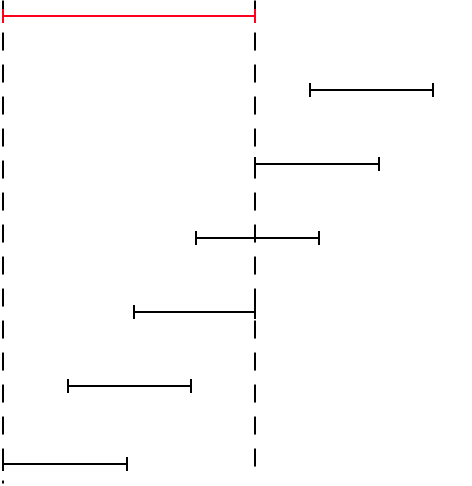
\includegraphics[height=2.02in]{intervals.png}}&\emph{equals} \{=\} &\\
    & &\\
                   &\emph{before} \{\textless\} / \emph{after} \{\textgreater\} & $\langle L \rangle$ / $\langle \overline{L} \rangle$ \emph{(Later)}\\
    & &\\
                   &\emph{meets} \{\emph{m}\} / \emph{met-by} \{\emph{mi}\} &$\langle A \rangle$ / $\langle \overline{A} \rangle$ \emph{(After)}\\
    & &\\
    &\emph{overlaps} \{\emph{o}\} / \emph{overlapped-by} \{\emph{oi}\} &$\langle O \rangle$ / $\langle \overline{O} \rangle$ \emph{(Overlaps)}\\
    & &\\
    &\emph{finished-by} \{\emph{fi}\} / \emph{finishes} \{\emph{f}\} &$\langle E \rangle$ / $\langle \overline{E} \rangle$ \emph{(Ends)}\\
    & &\\
    &\emph{contains} \{\emph{di}\} / \emph{during} \{\emph{d}\} &$\langle D \rangle$ / $\langle \overline{D} \rangle$ \emph{(During)}\\
    & &\\
    &\emph{started-by} \{\emph{si}\} / \emph{starts} \{\emph{s}\} &$\langle B \rangle$ / $\langle \overline{B} \rangle$ \emph{(Begins)}
  \end{tabular}
\end{table}
\subsubsection{Propp Example with Punch and Judy}
In this example, we combine Halpern and Shoham's temporal operators with the possibility ($\Diamond$) and necessity ($\Box$) operators of modal logic. We follow the convention of writing possibility operators inside angle brackets: $\langle \, \rangle$ and necessity operators within square brackets: $[ \, ]$.

This example shows the ``sausages'' scene described in section \ref{sec:pjexample}, consisting of a set of situations $S$, containing Propp story functions $P$. The interval temporal logic operators used in this example are the set $T$. Figure \ref{fig:operators} shows the modal operators we use. $A, B$ and $C$ in formula \ref{eq:story} are variables that represent the characters and objects that appear in the story.
\begin{figure}[!t]
\begin{align}
    S &= \{S_0, S_1, S_2, S_{3a}, S_{3a_1}, S_4, S_{3b}, S_{3b_1}, S_4, S_5\}\\
    P &= \{\mathtt{interdiction(A, B, C), absentation(A), struggle(A, B),}\nonumber\\
  &\qquad\qquad\mathtt{victory(A), villainy(A, B), violation(A, B), return(A)}\}\label{eq:story}\\
  T &= \{D, \overline{D}, O, \overline{O}, A, \overline{A}, B, \overline{B}, L, \overline{L}, E, \overline{E}\}
\end{align}
\caption{Modal operators}\label{fig:operators}
\end{figure}
Hybrid logics allow worlds, time intervals, to be named. The hybrid logic nominal operator allows specific times to be uniquely referenced, allowing a logic to talk about specific states such as $S_0..S_5$. The nominal proposition is true of one specific time interval such that any two worlds with the same name represent co-extensive intervals of time. Anything true of one is true of the other.
We also make use of a nominal modal operator so that it is possible to make assertions about these named worlds, ``It is necessary that in state $S_1$ Joey absents himself.'' This technique enables us to associate story functions with specific, named intervals.
We use hybrid logic to identify nodes using the \emph{nominal} operator, shown as $@$. The nominal operator adds the capability of referring to possible worlds in formulas. In this way, each possible state of a system can be labelled and referenced from other states. As seen in figure \ref{fig:lotrec}, each nominal node must have its own name as a relation leading back to the root node, in order to be linked to and referred from the other nodes.
We can combine this with the Interval Temporal Logic to make statements such as ``An absentation starts with state $@S_1$ and ends with state $@S_5$.'' (formula \ref{eq:absentation}).
Figure \ref{fig:situations} describes the full sausages scene from Punch and Judy using the time intervals shown in figure \ref{fig:durations}.
\begin{figure}[!t]
  \centering
    \centerline{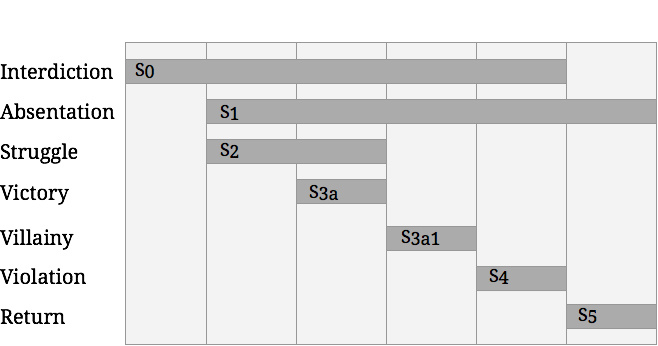
\includegraphics[width=0.9\textwidth]{durations.png}}
  \caption{Timings of the story functions in the sausages scene}\label{fig:durations}
\begin{align}
  &S_{0} \land \mathit{interdiction(Joey, Punch, Sausages)} \land\nonumber\\
  &\qquad\qquad\qquad\qquad\qquad\langle B \rangle @S_{1} \land \langle E \rangle @S_{4} \land \langle A \rangle @S_{5}\label{eq:interdiction}\\
  &[@S_{1}] \mathit{absentation(Joey)} \land \langle A \rangle @S_{2}\label{eq:absentation}\\
  &[@S_{2}] \mathit{struggle(Punch, Crocodile)} \land \langle E \rangle (@S_{3a} \lor @S_{3b})\label{eq:struggle}\\
  &[@S_{3a}] \mathit{victory(Crocodile)} \land \langle A \rangle @S_{3a_1}\\
  &[@S_{3a_1}] \mathit{villainy(Crocodile, Sausages)} \land \langle E \rangle @S_{4}\\
  &[@S_{3b}] \mathit{victory(Punch)} \land \langle A \rangle @S_{3b_1}\\
  &[@S_{3b_1}] \mathit{villainy(Punch, Sausages)} \land \langle E \rangle @S_{4}\\
  &[@S_{4}] \mathit{violation(Punch, Sausages)}\\
  &[@S_{5}] \mathit{return(Joey)}
\end{align}
\caption{Sausages scene with nominals and Interval Temporal Logic}\label{fig:situations}
\end{figure}

One notable feature of this approach is that it enables the building of reusable story components. For example, we have said that an interdiction must begin with an absentation and ends with a violation (formula \ref{eq:interdiction}). This pattern can be reused in different stories, or several times in the same story. Additionally, it allows for the abstraction and combination of story components in a more expressive way than Propp's original story functions. This is because Propp only describes narrative events at one level of abstraction. For example, he describes stories as a series of events containing an interdiction followed by an absentation, followed by a violation. But there is no mechanism for combining these three functions into a higher-level component (which could be called ``Don't do that, or else!'', for example). Our approach makes such abstraction and recombination possible.

\section{Describing Punch and Judy with Kripke Structures}\label{sec:kripke}
\begin{figure}[!t]
  \centering
    \centerline{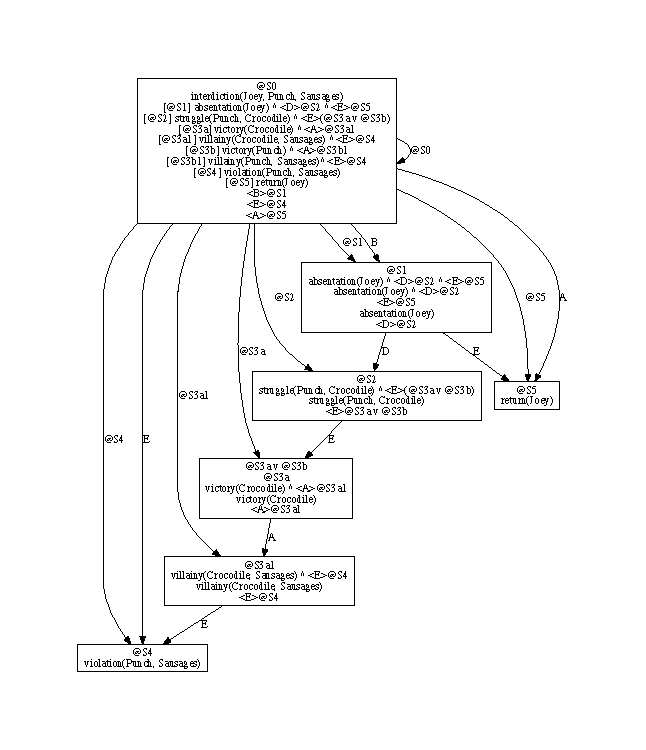
\includegraphics[width=0.9\textwidth]{crocmodel.pdf}}
  \caption{One model from the sausages scene in LoTREC}\label{fig:lotrec}
\end{figure}

We use Kripke structures \cite{kripke1963semantical} as a method of interpreting the combination of modal logic with Interval Temporal Logic. A Kripke structure is a graph, the nodes of which represent a possible world consisting of a set of assertions, and the edges of which are the accessibility relations between worlds.

\subsubsection{LoTREC}
% Read the book
In order to build and visualise the Kripke structures, we use LoTREC \cite{del2001lotrec}, a generic tableaux prover for modal and description logics. It allows the user to build up Kripke models using a domain specific language and display those models in the form of a graph diagram.
LoTREC uses the tableau method for model checking. This method checks whether or not its input is satisfiable by attempting to build a model for it. If the model construction fails, then the input is unsatisfiable.
Building models in LoTREC consists of defining \emph{connectors}, \emph{rules} and \emph{strategies}. Connectors are the logical operators used in formulas, rules are the instructions LoTREC needs to expand them into new nodes and edges and strategies are ways of combining rules in order to form models.
LoTREC takes an initial set of formulas as input and expands each formula into its components. These formulas are input using a simple prefix notation domain specific language consisting of operators and arguments, described in the LoTREC instruction book \emph{Kripke's Worlds} \cite{gasquet2013kripke}.
In the expansion, if a $[\,]$ (necessary) operator is encountered, then the formulas that serve as its argument are propagated across to all subsequent nodes. In the case of a $\langle \, \rangle$ (possibility) operator, a new node (possible world) is created containing its arguments. In both cases, binary operators can be used where one argument is located inside the square or angle brackets. In these cases, the argument inside the brackets is the accessibility relation, and is used to label the edges leading to the subsequent nodes.
In the case of a disjunction ($\lor$) operator, the current model is copied in its entirety and extended with one of the operator's arguments. The other argument is added onto the current model. This is an important way of creating alternative routes through the narrative, all of which can be checked for consistency.

\paragraph{The Sausages Scene in LoTREC}
The narrative is captured as a system of interval temporal logic assertions over story functions. The  assertions are interpreted using a tableaux reasoner by unpacking them to form a Kripke structure.
Using the initial formulas from figure \ref{fig:situations} as input, figure \ref{fig:lotrec} shows the model for the case where Punch wins the fight with the Crocodile. One other model exists in this scenario, in which the Crocodile is instead the victor.

The example in figure \ref{fig:lotrec} describes the fabula of a branching story, where either Punch or the Crocodile may win the fight for the sausages. This corresponds to the disjunction in figure \ref{fig:situations}, formula \ref{eq:struggle}. This leads to the creation of two models: the one in which the Crocodile wins and then goes on to eat the sausages (situation $@S_{3a}$), and the one in which Punch wins (situation $@S_{3b}$).
Using a breadth first strategy like LoTREC we would build all models simultaneously. This enables them to be checked for internal consistency, eliminating potentially impossible temporal arrangements. For example, no interval may come after or later than itself.

The first node contains the logical description of the story, which is then unpacked into subsequent nodes. It starts with the initial situation, $S_0$, which contains an interdiction: $\mathit{interdiction(Joey, Punch, Sausages)}$, where Joey tells Punch to look after the sausages. The other situations, $S_1$ to $S_5$ are listed using the necessity operator, with their accessibility relations being each situation's nominal operator (such as $@S_1$). This means that these situations are all created as new nodes, linked to the root node using their nominal accessibility relation, and so can be referred to later using the nominal operator. In this way, situations can refer to other situations.

For example, in Propp's formalism, an interdiction must begin with the absentation of a character and end with the interdiction's violation. For this reason, the initial situation is connected to $@S_1$, ($\mathit{absentation(Joey)}$), with the $\langle B \rangle$ (begins) accessibility relation and to $@S_4$, ($\mathit{violation(Punch, Sausages)}$), with the $\langle E \rangle$ (ends) accessibility relation. As other situations are unpacked into nodes, they are linked to other situations in the same way. An example of this is shown in $S_1$, the absentation, which must end with Joey's return, $S_5$, and during which a struggle must occur ($S_2$). As the formulas inside $S_1$ are unpacked, $S_1$ is linked to the other situations with the appropriate temporal accessibility relations. This is all made possible with the hybrid logic, which allows nodes to be referred to by name and linked to.

By describing situations that are linked together with temporal relations, we can build narratives and check them as we go. If a narrative is inconsistent in some way (by stating that a character is both dead and alive, for example), then the model will be unsatisfiable. This is useful for ensuring the construction of consistent narratives.

Additionally, every time a story has the possibility of branching off, the model for each new branch can be checked to see if it is viable in the narrative world. This means that rather than relying on an author to write out each branch of a story, they can be generated automatically from a story description and checked for inconsistencies.

As mentioned previously, the combination of Interval Temporal Logic and a narrative formalism such as Propp's allows us to create abstracted story components. For example, we have described the interdiction as being started by an absentation and ended with a violation. This pattern can be called the ``interdiction pattern'', and so can be easily reused in other narratives.

The use of LoTREC has shown the utility of being able to visualise a branching narrative in its entirety. This suggests that our method enables the visual authoring of interactive narratives by non-technical creators. Rather than having to type in computer code, or logical formulas, a visual tool could be developed to create logically consistent narrative worlds.

This approach for describing narrative has many potential real-world uses. One obvious use would be for computer game narratives, but it could also be used to describe a repeatable training scenario, and the possible choices available to a user at any point during the simulation.

\subsection{Deontic Logic and Norms}

\section{Norms and Institutions}
\label{sec:norms-and-institutions}

An institution describes a set of `social' norms describing the permitted and obliged behaviour of interacting agents. Noriega's `Fish Market' thesis~\cite{noriega1999agent} describe how an institutional model can be used to regiment the actions of agents in a fish market auction. Several~\cite{artikis2009specifying,fornara2007agent,cardoso2007institutional} extend this idea to build systems where institutions actively regulate the actions of agents, while still allowing them to decide what to do. We build on the work of Cliffe et al.~\cite{cliffe2007specifying} and Lee et al.~\cite{lee2013decoupling} to adapt it for the world of narrative, using an institutional model to describe the story world of Punch and Judy in terms of Propp's story moves and character roles, through which the actors acquire powers and permissions appropriate to the character and the story function in which they are participating.

Institutional models use concepts from deontic logic to provide obligations and permissions that act on interacting agents in an environment. By combining this approach with Propp's concepts of \emph{roles} and \emph{story moves}, we describe a Propp-style formalism of Punch and Judy in terms of what agents are \emph{obliged} and \emph{permitted} to do at certain points in the story.

For example, in one Punch and Judy scene, a policeman enters the stage and attempts to apprehend Punch. According to the rules of the Punch and Judy world, Punch has an obligation to kill the policeman by the end of the scene (as this is what the audience expects to happen, having seen other Punch and Judy shows). The policeman has an obligation to try his best to catch Punch. Both agents have permission to be on the stage during the scene. The policeman only has permission to chase Punch if he can see him (Punch is obliged to hide from him at the start of the scene).

The permissions an agent has, on the one hand, constrain the choices of actions available to them at any given moment. Obligations, on the other hand, affect the goals of an agent. Whether or not an agent actively tries to fulfil an obligation depends on their emotional state.

\subsection{Institution example}
To illustrate the application of institutional modelling, we here continue the `sausages and crocodile' scene example from section~\ref{sec:pjexample}, taking the Propp story functions and describing them in an institutional model.  We define our institution in terms of \emph{fluents}, \emph{events}, \emph{powers}, \emph{permissions} and \emph{obligations}, following~\cite{cliffe2007specifying}, to which the interested reader is referred for the full details of the formal model, including the generate ($\cal G$) and consequence ($\cal C$) relations, which are only described here in sufficient depth for the model being presented.

\subsubsection{Fluents}
These are properties that may or may not hold true at some instant in time, and that change over the course of time. \emph{Institutional events} are able to \emph{initiate} or \emph{terminate} fluents at points in time. A fluent could describe whether a character is currently on stage, the scene of the story that is currently being acted out, or whether or not the character is happy at that moment in time.
Domain fluents ($\mathcal{D}$) describe domain-specific properties that can hold at a certain point in time. In the Punch and Judy domain, these can be whether or not an agent is on stage, or their role in the narrative: % (equation~\ref{eq:domain}).
\begin{align*}
   \mathcal{D} &= \left\{\mathtt{onstage, hero, villain, victim, donor, item}\right\} %\label{eq:domain}
\end{align*}

Institutional fluents consist of (institutional) \emph{powers}, \emph{permissions} and \emph{obligations}.
% check your facts on this one
An \textbf{institutional power} ($\mathcal{W}$) describes whether or not an external event has the authority to generate a meaningful institutional event. Taking an example from Propp's formalism, an \emph{absentation\/} event can only be generated by an external event brought about by a \emph{donor\/} character (such as their leaving the stage). Therefore, any characters other than the donor character would not have the institutional power to generate an \emph{absentation\/} institutional event when they leave the stage.
The possible empowerments (institutional events) from Propp used in Punch and Judy are:
\begin{align*}
  \mathcal{W} =&\left\{\mathtt{pow(introduction), pow(interdiction), pow(give),}\right.\\ %\nonumber\\
               &\left. {} \mathtt{pow(absentation), pow(violation), pow(return)}\right\} %\label{eq:power}
\end{align*}

\subsubsection{Permissions} ($\mathcal{P}$) are associated with external actions that agents are permitted to do at a certain instant in time. These can be thought of as the set of \emph{socially permitted\/} actions available to an agent. While it is possible for an agent to perform other actions, societal norms usually discourage them from doing so.
% PJ examples
For example, it would not make sense in the world of Punch and Judy if Punch were to give the sausages to the Policeman. It is always Joey who gives the sausages to Punch. Also, it would be strange if Joey were to do this in the middle of a scene where Punch and Judy are arguing. We make sure agents' actions are governed so as to allow them only a certain subset of permitted actions at any one time. The set of permission fluents is:
\begin{align*}
\mathcal{P} =& \left\{\mathtt{perm(leavestage), perm(enterstage), perm(die), perm(kill),}\right.\nonumber\\
             &\left. {} \mathtt{perm(hit), perm(give), perm(fight)}\right\} %\label{eq:perm}
\end{align*}

\subsubsection{Obligations} ($\mathcal{O}$) are institutional facts that contain actions agents \emph{should} do before a certain deadline. If the action is not performed in time, a \emph{violation event} is triggered, which may result in a penalty being incurred. While an agent may be obliged to perform an action, it is entirely their choice whether or not they actually do so. They must weigh up whether or not pursuing other courses of action is worth accepting the penalty that an unfulfilled obligation brings.

% replace with sausages obligation
Anybody who has seen a Punch and Judy show knows that at some point Joey tells Punch to guard some sausages, before disappearing offstage. Joey's departure is modelled in the institution as the \emph{absentation\/} event. It could also be said that Joey has an obligation to leave the stage as part of the \emph{absentation} event, otherwise the story function is violated. This can be described in the institution as:
\begin{align*}
  \mathcal{O} =& \left\{\text{obl}(\mathtt{leavestage, absentation, viol(absentation)})\right\}%\label{eq:obl}
\end{align*}
The first argument is the external event that must be triggered according to the obligation, the second argument is the institutional deadline event, and the third argument is the violation event which is triggered if the obligation is not fulfilled before the deadline. 

\subsubsection{Events}
% actually 3 kinds, including violation events
Cliffe's model specifies three types of \textbf{event}: \emph{external events} (or `observed events', $\mathcal{E}_{obs}$), \emph{institutional events} ($\mathcal{E}_{instevent}$) and \emph{violation events} ($\mathcal{E}_{viol}$). Examples of each are given in Figure~\ref{fig:events}.
\emph{External events} are observed to happen in the agents' environment, which can \emph{generate} \emph{institutional events} which occur only within the institional model, leading to the \emph{initiation} or \emph{termination} of (domain) fluents, permissions, obligations or institutional powers.
An external event could be an agent leaving the stage, an agent hitting another, or an agent dying. Internal events include narrative events such as scene changes, or the triggering of Propp story functions such as \emph{absentation} or \emph{interdiction} (described in section~\ref{sec:propp}). \emph{Violation} is the name of a Propp story function, and is included as an internal event, although it has no relation to the violation events of an institution.
Violation events occur when an agent has failed to fulfil an obligation before the specified deadline. These can be implemented in the form of a penalty, by decreasing an agent's health, for example.

\begin{figure}[!t]
\begin{align}
  \mathcal{E}_{obs} =& \left\{\mathtt{startshow, leavestage, enterstage, die, give,}\right.\nonumber\\
  &\left. {} \mathtt{harmed, hit, fight, kill, escape}\right\}\label{eq:eobs}\\
  \mathcal{E}_{instevent} =& \left\{\mathtt{introduction, interdiction, receipt, absentation,}\right.\nonumber\\
                         &\left. {} \mathtt{violation, return, struggle, defeat, complicity,}\right.\nonumber\\
                         &\left. {} \mathtt{victory, escape}\right\}\label{eq:einst}\\
  \mathcal{E}_{viol} =& \left\{\mathtt{viol(introduction), viol(interdiction), viol(receipt),}\right.\nonumber\\
 &\left. {} \mathtt{viol(absentation), viol(violation), viol(return),}\right.\nonumber\\
 &\left. {} \mathtt{viol(struggle), viol(defeat), viol(complicity)}\right.\nonumber\\
 &\left. {} \mathtt{viol(victory), viol(escape)}\right\}\label{eq:viol}
\end{align}
\caption{External, institutional and violation events for Punch and Judy} \label{fig:events}
\end{figure}

% internal and external

\subsubsection{Event Generation and Consequences}
An \textbf{event generation} function, $\mathcal{G}$, describes how events
($\mathcal{E}$, usually external, but can also be internal) %\mnote{Added $\mathcal{E}$ explanation here}
can generate other (usually institutional) events, conditional upon the current institutional state ($\cal X$). This is the counts-as relation.  For example, if an agent leaves the stage while the \emph{interdiction} event holds, they trigger the \emph{leavestage} event. This combination generates the \emph{absentation} institutional event (rule~\ref{eq:absentation}). Further examples appear in figure~\ref{fig:gen}.

Event generation functions follow a $\langle \mathtt{preconditions} \rangle \rightarrow \{\mathtt{postconditions}\}$ format. The preconditions consist of a set of fluents that hold at that time, along with an event to have occurred. The postconditions are the events that are generated. The generation functions are used to generate internal, institutional events from external events.

Consider the Punch and Judy scenario described in section~\ref{sec:pjexample}. There are seven institutional events (story functions) that occur during this scene: \emph{interdiction}, \emph{complicity}, \emph{receipt} (from Propp's \emph{receipt of a magical agent}) \emph{absentation}, \emph{violation}, \emph{struggle}, \emph{return}.
These institutional events are all generated by external events. The \emph{interdiction} is generated when Joey tells Punch to protect the sausages. Punch agreeing amounts to \emph{complicity}. Joey \emph{gives} punch the sausages (\emph{receipt}), then leaves the stage (\emph{absentation}). The crocodile eating the sausages is a \emph{violation} of Punch's oath, the agents fight (\emph{struggle}), then Joey enters the stage again (\emph{return}).

It is desirable that these story functions occur in this sequence in order for a satisfying narrative to emerge. Agents may decide to perform actions that diverge from this set of events, but the institution is guiding them towards the most fitting outcome for a \emph{Punch and Judy} world. For this reason, a currently active story function can be the precondition for event generation. For example, the \emph{receipt} event may only be triggered if an agent externally performs a \emph{give} action \textbf{and} if the \emph{complicity} event currently holds (rule~\ref{eq:receipt}).
Examples of event generation function for this scenario, complete with preconditions, are listed in rules~\ref{eq:gfirst}--\ref{eq:glast} (Figure~\ref{fig:gen}).

\begin{figure}[!t]
\abovedisplayskip=0pt
\abovedisplayshortskip=0pt
$\mathcal{G(X, E)}:\left\{\mbox{%
{\begin{minipage}[c]{0.85\textwidth}
% \vspace{-2.1em}\begin{align}
\begin{align}
\langle \emptyset,\mathit{tellprotect}\mathtt{(donor, villain, item)} \rangle%\nonumber\\
             %         &\qquad\qquad\qquad
& \rightarrow \left\{\mathit{interdiction}\right\}\label{eq:gfirst}\\
                      \langle \{\mathit{interdiction}\}, \mathit{agree}\mathtt{(villain)}) \rangle %\nonumber\\
            %          &\qquad\qquad\qquad
& \rightarrow \left\{\mathit{complicity}\right\}\\
                      \langle \emptyset, \mathit{give}\mathtt{(donor, villain, item)}) \rangle %\nonumber\\
        %              &\qquad\qquad\qquad
& \rightarrow \left\{\mathit{receipt}\right\}\label{eq:receipt}\\
                      \langle \{\mathit{interdiction}\}, \mathit{leavestage}(\mathtt{donor}) \rangle %\nonumber\\
              %        &\qquad\qquad\qquad
& \rightarrow \left\{\mathit{absentation}\right\}\label{eq:absentation}\\
                      \langle \{\mathit{interdiction}\}, \mathit{harmed}(\mathtt{item}) \rangle %\nonumber\\
         %             &\qquad\qquad\qquad
& \rightarrow \left\{\mathit{violation}\right\}\\
                      \langle \{\mathit{interdiction, absentation}\},
                      \mathit{enterstage}(\mathtt{donor}) \rangle %\nonumber\\
              %        &\qquad\qquad\qquad
& \rightarrow \left\{\mathit{return}\right\}\\
                      \langle \emptyset, \mathit{hit}(\mathtt{donor, villain}) \rangle %\nonumber\\
%                      &\qquad\qquad\qquad
& \rightarrow \left\{\mathit{struggle}\right\}\label{eq:glast}
\end{align}
\end{minipage}}}\right.$
\caption{Event generation in the sausage scene} \label{fig:gen}
\end{figure}

\textbf{Consequences} consist of fluents, permissions and obligations that are \emph{initiated} ($\mathcal{C}^{\uparrow}$) or \emph{terminated} ($\mathcal{C}^{\downarrow}$) by institutional events. For example, the institutional event \emph{receipt} initiates the donor agent's permission to leave the stage, triggering the \emph{absentation} event (rule~\ref{eq:initgive}). When the \emph{interdiction} event is currently active and a \emph{violation} event occurs, the interdiction event is terminated (\ref{eq:interm}). Rules~\ref{eq:cfirst}--\ref{eq:clast} in Figures~\ref{fig:init} and~\ref{fig:term} describe the initiation and termination of fluents in the Punch and Judy sausages scene detailed in section~\ref{sec:pjexample}.

\begin{figure}[!t]
\abovedisplayskip=0pt
\abovedisplayshortskip=0pt
$\mathcal{C^{\uparrow}(X, E)}:\left\{\mbox{%
\begin{minipage}[c]{0.85\textwidth}
\begin{align}
    \langle \emptyset, \mathtt{interdiction} \rangle %\nonumber\\
                                 % &\qquad\qquad
&\rightarrow \{\text{active}(\mathtt{interdiction}), \nonumber\\&\qquad\text{perm}(\mathtt{give(donor, villain, item)})\}\label{eq:cfirst}\\
                                 \langle \emptyset, \mathtt{receipt} \rangle % \nonumber\\
                                 % &\qquad\qquad
&\rightarrow \{\text{perm}(\mathtt{leavestage(donor)})\}\label{eq:initgive}\\
                                 \langle\{\mathit{active(absentation)}\}, \nonumber\\\mathtt{enterstage(villain)} \rangle %\nonumber\\
                                 %&\qquad\qquad
&\rightarrow \{\text{obl}(\mathtt{eat(villain, sausages),} \nonumber\\&\qquad\qquad\mathtt{return, viol(violation)})\}\label{eq:obl1}\\
                                 \langle\{\mathit{active(interdiction)}\}, \nonumber\\\mathtt{leavestage(donor)} \rangle % \nonumber\\
                                 % &\qquad\qquad
&\rightarrow \{\text{obl}(\mathtt{enterstage(donor),}\nonumber\\&\qquad\qquad\mathtt{eat(villain, sausages),}\nonumber\\&\qquad\qquad\mathtt{viol(return)})\}\label{eq:obl2}\\
                                 \{\mathit{active(interdiction)}\},\nonumber\\ \mathtt{violation} \rangle %\nonumber\\
                                 % &\qquad\qquad
&\rightarrow \{\text{perm}(\mathtt{enterstage(dispatcher)})\}\\
                                 \langle\{\mathit{active(absentation),}\nonumber\\\mathit{active(violation)}\},\nonumber\\ \mathtt{return} \rangle %\nonumber\\
                                 %&\qquad\qquad
&\rightarrow \{\text{perm}(\mathtt{hit(donor, villain)})\}
\end{align}
\end{minipage}}\right.$
\caption{Fluent initiation in the sausage scene} \label{fig:init}
\medskip
\abovedisplayskip=0pt
\abovedisplayshortskip=0pt
$\mathcal{C^{\downarrow} (X, E)}:\left\{\mbox{%
\begin{minipage}[c]{0.85\textwidth}
\begin{align}
\langle \emptyset, \mathtt{interdiction} \rangle %\nonumber\\
                                   %&\qquad\qquad
&\rightarrow \{\text{perm}(\mathtt{give(donor, villain, item)})\}\\
                                   \langle \{\mathit{active(interdiction)}\},\nonumber\\ \mathtt{absentation} \rangle %\nonumber\\
                                   %&\qquad\qquad
&\rightarrow \{\text{perm}(\mathtt{leavestage(donor)})\}\\
                                   \langle \{\mathit{active(interdiction)}\},\nonumber\\ \mathtt{violation} \rangle %\nonumber\\
                                   %&\qquad\qquad
&\rightarrow \{\mathit{active(interdiction)}\}\label{eq:interm}\\
                                   \langle \{\mathit{active(absentation),}\nonumber\\\mathit{ active(violation)}\},\nonumber\\ \mathtt{return} \rangle %\nonumber\\
                                   %&\qquad\qquad
&\rightarrow \{\mathit{active(absentation)}\}\label{eq:clast}
\end{align}
\end{minipage}}\right.$
\caption{Fluent termination in the sausage scene} \label{fig:term}
\end{figure}%\mnote{Added \emph{active(interdiction)} to top of fig. \ref{fig:init}}

\section{Why Use Institutions for Interactive Narrative?}
\label{sec:why-use-institutions}
% Write about character freedom, regimentation vs regulation. Give story
% examples vs using a planner

\chapter{Tropes as Story Components}
\label{cha:tropes}
\section{Tropes: a ``Folksonomy'' of Story Components}
% Describe TVtropes

\section{Why Use Tropes?}
% Write about ability to abstract, give story examples vs Propp

\chapter{Describing Story Worlds with Tropes and Institutions}
\label{cha:tropes-and-institutions}

\chapter{Future Work}
\label{cha:future}


\bibliographystyle{apalike}
\bibliography{thesis}

\end{document}